\subsection{Class Diagram}
\begin{center}
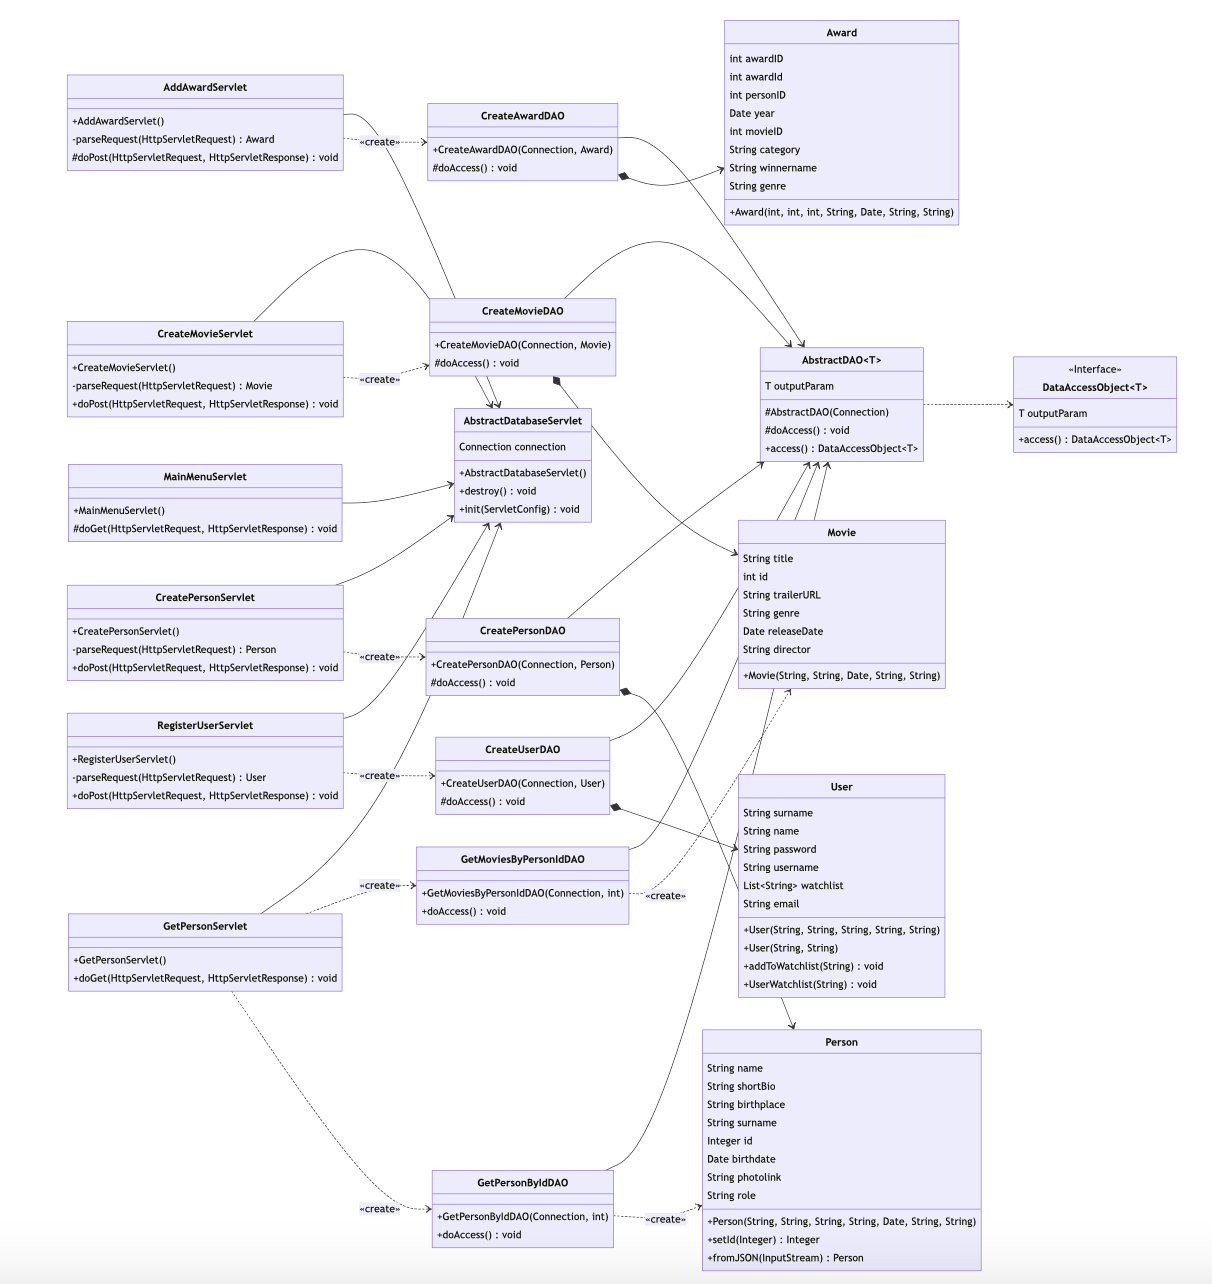
\includegraphics[angle=0, width=1.07\textwidth]{pictures/umlar.png}
\end{center}
%Describe here the class diagram of your project
\bigskip
The class diagram contains (some of) the classes used to handle User, Movie, Person, and Award. We describe several servlets: MainMenuServlet which retrieves the information of a movie and awards, and the CreateMovieServlet which handles the Movie resource and allows to creation of a movie. Similarly, CreatePersonServlet handles the Person resource and allows the creation of a person according to the attributes it has. Each servlet extends the AbstractDatabaseServlet which is needed to acquire the connection to the database. The movie resource is handled by two servlets CreateMovieServlet and MoviePageServlet: these servlets implement doPost and doGet methods accordingly.
Existing user's login operation is handled by UserLoginServlet and RegisterUserServlet handles the registration operation of a new user.
The MovieDAO class interacts with the database to retrieve movie information and CreateMovieDAO creates a new movie resource, while the GetMovieByPersonIdDAO class allows to retrieve the information about a movie given the PersonId (in this case the director, actor, or any other role).
Each DAO class extends the AbstractDAO class (which is delegated to the interaction with the database) and defines the doAccess() method. The AbstractDAO class implements the DataAccessObject interface. 

